\documentclass[10pt,a4paper]{article}
\usepackage[margin=22mm]{geometry}
\usepackage[T1]{fontenc}
\usepackage{lmodern,amsmath,amssymb,booktabs,graphicx,tikz,hyperref,fvextra}
\usetikzlibrary{arrows.meta,positioning,calc,decorations.pathmorphing}
\definecolor{ink}{RGB}{20,53,78}
\hypersetup{colorlinks=true,urlcolor=ink,linkcolor=ink}
\setlength{\parindent}{0pt}
\setlength{\parskip}{5pt}
\emergencystretch=3em

\title{\color{ink}Ventilation as a bilinear dynamical system}
\author{}
\date{Original learning collection -- November 2026}
\begin{document}
\begin{center}{\LARGE\color{ink}Ventilation as a bilinear dynamical system}\\[5pt]{\small Original learning collection -- November 2026}\end{center}

\textbf{Evidence note.} Original teaching scenario. Numerical parameters are deliberately chosen for learning. All generated data and curves are synthetic; no physical measurement is asserted.
\section{Design brief}
A hypothetical well-mixed room has $V=120\,\mathrm{m^3}$, tracer generation $S=360\,\mathrm{ppm\,m^3/min}$ and nominal airflow $q_0=3\,\mathrm{m^3/min}$. Inlet excess concentration is zero. Derive the equilibrium and local airflow-to-concentration model from $V\dot c=S-qc$. Compare $10\%$ and $100\%$ airflow increases using the nonlinear and linearized models, including their final-value errors.
\section{Physical system}
\begin{center}\resizebox{\ifdim\width>.98\linewidth.98\linewidth\else\width\fi}{!}{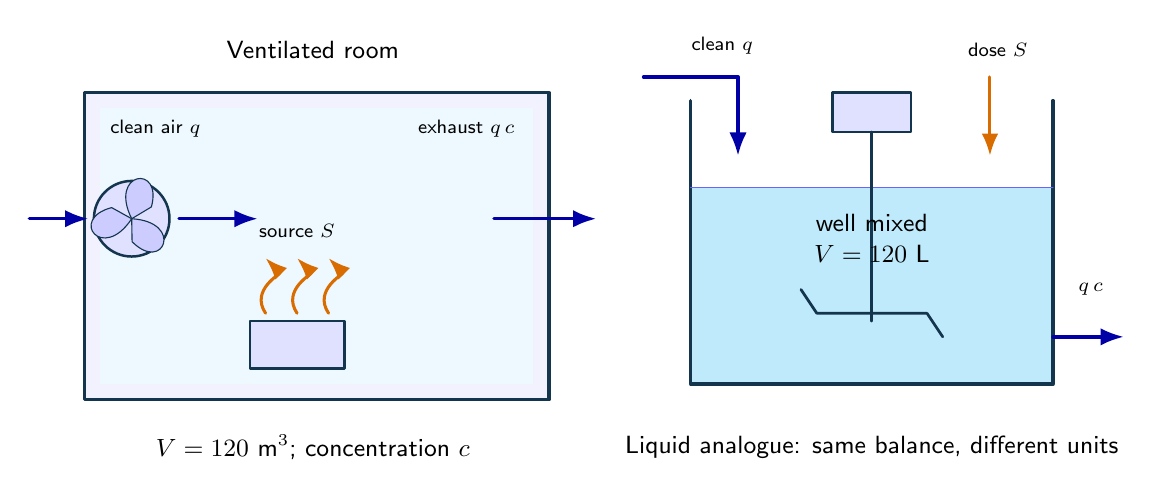
\begin{tikzpicture}[
font=\sffamily\small,>=Latex,line cap=round,line join=round,
wall/.style={draw=ink,line width=1.2pt,fill=blue!5},
water/.style={fill=cyan!25,draw=none},
metal/.style={draw=ink,fill=blue!12,line width=.9pt},
flow/.style={->,draw=blue!65!black,line width=1.2pt},
heat/.style={->,draw=orange!85!black,line width=1.1pt},
measure/.style={->,draw=teal!70!black,line width=.9pt},
dim/.style={<->,draw=ink!65,line width=.6pt},
spring/.style={draw=ink,decorate,decoration={coil,aspect=.5,segment length=4pt,amplitude=3pt}},
wire/.style={draw=ink,line width=1pt},
lab/.style={align=center,font=\sffamily\small},
smalllab/.style={align=center,font=\sffamily\scriptsize}]

\draw[wall](.3,.2)--(.3,4.1)--(6.2,4.1)--(6.2,.2)--cycle;
\fill[cyan!7](.5,.4)rectangle(6,3.9);
\draw[metal](.9,2.5)circle(.48);
\foreach \a in {0,120,240}{\draw[ink,fill=blue!20,rotate around={\a:(.9,2.5)}](.9,2.5)..controls(.6,3.1)and(1.3,3.2)..(1.15,2.65)--cycle;}
\draw[flow](-.4,2.5)--(.35,2.5);
\draw[flow](1.5,2.5)--(2.5,2.5);
\draw[flow](5.5,2.5)--(6.8,2.5);
\node[smalllab]at(1.2,3.65){clean air $q$};
\node[smalllab]at(5.15,3.65){exhaust $q\,c$};
\draw[metal](2.4,.6)rectangle(3.6,1.2);
\foreach \x in {2.6,3,3.4}{\draw[heat](\x,1.3)..controls(\x-.2,1.6)and(\x+.2,1.8)..(\x,2);}
\node[smalllab]at(3,2.35){source $S$};
\node[lab]at(3.2,4.65){Ventilated room};
\node[lab]at(3.2,-.4){$V=120$ m$^3$; concentration $c$};
\fill[water](8,.4)rectangle(12.6,2.9);
\draw[wall,fill=none](8,4)--(8,.4)--(12.6,.4)--(12.6,4);
\draw[blue!60](8,2.9)--(12.6,2.9);
\draw[flow](7.4,4.3)--(8.6,4.3)--(8.6,3.3);
\draw[flow](12.6,1)--(13.5,1);
\draw[metal](9.8,3.6)rectangle(10.8,4.1);
\draw[wire](10.3,3.6)--(10.3,1.2);
\draw[wire](9.6,1.3)--(11,1.3)(9.6,1.3)--(9.4,1.6)(11,1.3)--(11.2,1);
\draw[heat](11.8,4.3)--(11.8,3.3);
\node[smalllab]at(11.9,4.65){dose $S$};
\node[smalllab]at(8.4,4.7){clean $q$};
\node[smalllab,anchor=west]at(12.8,1.6){$q\,c$};
\node[lab]at(10.3,2.25){well mixed\\$V=120$ L};
\node[lab]at(10.3,-.4){Liquid analogue: same balance, different units};
\end{tikzpicture}
}\par{\small A ventilated room and a well-mixed liquid analogue share an inventory balance. The room uses m$^3$ and the liquid case uses L; do not mix their concentration or flow units. Equal inlet and outlet volume flows keep each inventory constant.}\end{center}
\section{Concentration balance}
For a perfectly mixed room, let $c$ be excess tracer concentration in ppm, $q$ ventilation flow in m$^3$/min and $S$ tracer generation in ppm m$^3$/min. Conservation gives
\[V\dot c=S-qc.\]
The model is bilinear in the two variables $q$ and $c$. At constant airflow $q_0=3$, the equilibrium is $c_0=S/q_0=120$ ppm.
\section{Local perturbation model}
Write $c=c_0+\delta c$ and $q=q_0+\delta q$. Expanding the product and subtracting the equilibrium gives
\[V\delta\dot c=-q_0\delta c-c_0\delta q-\delta q\delta c.\]
Discarding only the second-order product yields
\[\frac{\delta C(s)}{\delta Q(s)}=\frac{-c_0/q_0}{(V/q_0)s+1}=\frac{-40}{40s+1}.\]
Increasing airflow reduces concentration, so the negative static gain has a physical meaning.
\section{Finite changes and approximation error}
For a flow step $\Delta q$, the exact response is
\[c(t)=\frac{S}{q_0+\Delta q}+\left(c_0-\frac{S}{q_0+\Delta q}\right)e^{-(q_0+\Delta q)t/V}.\]
The local prediction is $c_{lin}(t)=c_0-40\Delta q(1-e^{-t/40})$. For a 10 percent step the exact final value is $120/1.1$ ppm, while the linear prediction is 108 ppm. For a doubling, they are 60 ppm and 0 ppm: a useful warning against extrapolating the tangent model.
\section{Interpretation}
The linearized model changes neither its time constant nor its input gain after a step. The nonlinear model changes both its equilibrium and decay rate. This is a tracer-transport teaching example, not an indoor-air-quality exposure assessment.
\section{What to learn from the experiment}
The doubled-flow experiment deliberately leaves the small-signal regime. Its large error is a limitation of linearization, not a numerical failure.
\section{System sketch}
\begin{center}\resizebox{\ifdim\width>.98\linewidth.98\linewidth\else\width\fi}{!}{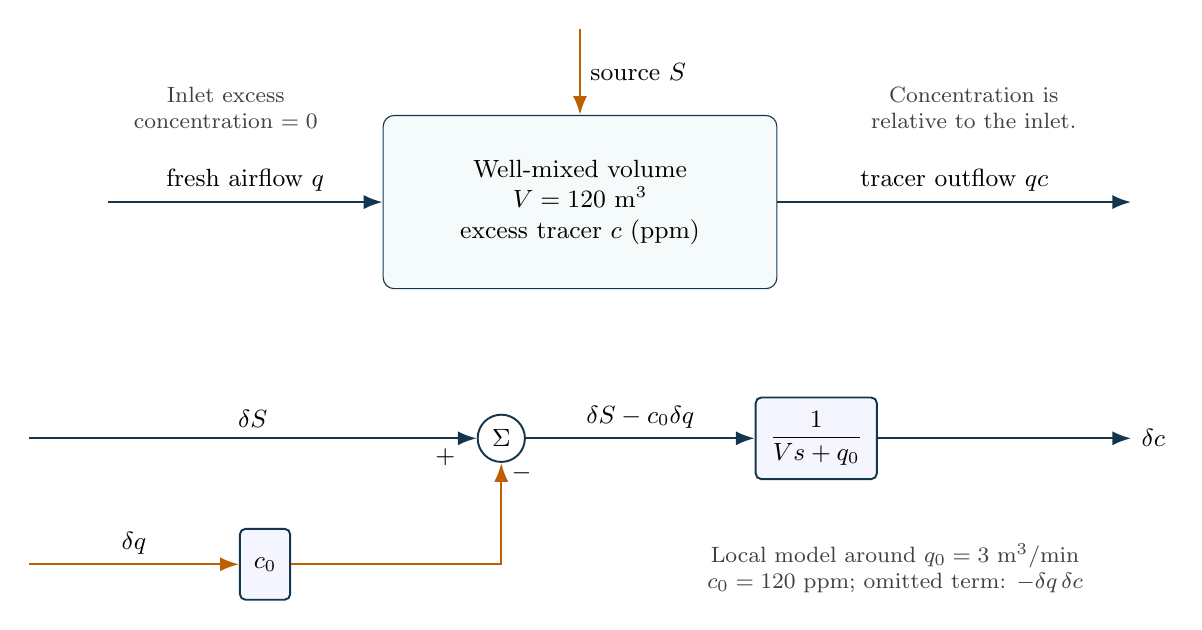
\begin{tikzpicture}[x=1cm,y=1cm,>=Latex,font=\small,
block/.style={draw=ink,fill=blue!4,rounded corners=2pt,minimum height=9mm,align=center,line width=.7pt,inner sep=5pt},
sum/.style={circle,draw=ink,fill=white,minimum size=6mm,inner sep=0pt,line width=.7pt},
sig/.style={->,draw=ink,line width=.85pt},
fb/.style={->,draw=teal!70!black,line width=.85pt},
dist/.style={->,draw=orange!75!black,line width=.85pt},
tap/.style={circle,fill=ink,inner sep=1.4pt},
note/.style={font=\footnotesize,align=center,text=black!75}]

\node[draw=ink,fill=teal!4,rounded corners,minimum width=50mm,minimum height=22mm,align=center](v)at(7,2.3){Well-mixed volume\\$V=120\ \mathrm{m^3}$\\excess tracer $c$ (ppm)};
\draw[sig](1,2.3)--node[above]{fresh airflow $q$}(v.west);
\draw[sig](v.east)--node[above]{tracer outflow $qc$}(14,2.3);
\draw[dist](7,4.5)--node[right]{source $S$}(v.north);
\node[note]at(2.5,3.5){Inlet excess\\concentration $=0$};
\node[note]at(12,3.5){Concentration is\\relative to the inlet.};
\node[sum](s)at(6,-.7){$\Sigma$};
\node[block](p)at(10,-.7){$\dfrac{1}{Vs+q_0}$};
\node[block](gain)at(3,-2.3){$c_0$};
\draw[sig](0,-.7)--node[above]{$\delta S$}node[pos=.93,below]{$+$}(s);
\draw[dist](0,-2.3)--node[above]{$\delta q$}(gain);
\draw[dist](gain)--(6,-2.3)--node[pos=.9,right]{$-$}(s);
\draw[sig](s)--node[above]{$\delta S-c_0\delta q$}(p);
\draw[sig](p)--(14,-.7)node[right]{$\delta c$};
\node[note]at(11,-2.35){Local model around $q_0=3\ \mathrm{m^3/min}$\\$c_0=120\ \mathrm{ppm}$; omitted term: $-\delta q\,\delta c$};

\end{tikzpicture}
}
\par\small\refstepcounter{figure}\label{fig:system}\textbf{Figure \thefigure.} The physical balance and its local two-input signal model. Airflow enters with a negative sign because increased ventilation removes excess tracer.\end{center}
\section{Executed computational evidence}
\VerbatimInput[fontsize=\small,breaklines=true]{results.txt}
\begin{center}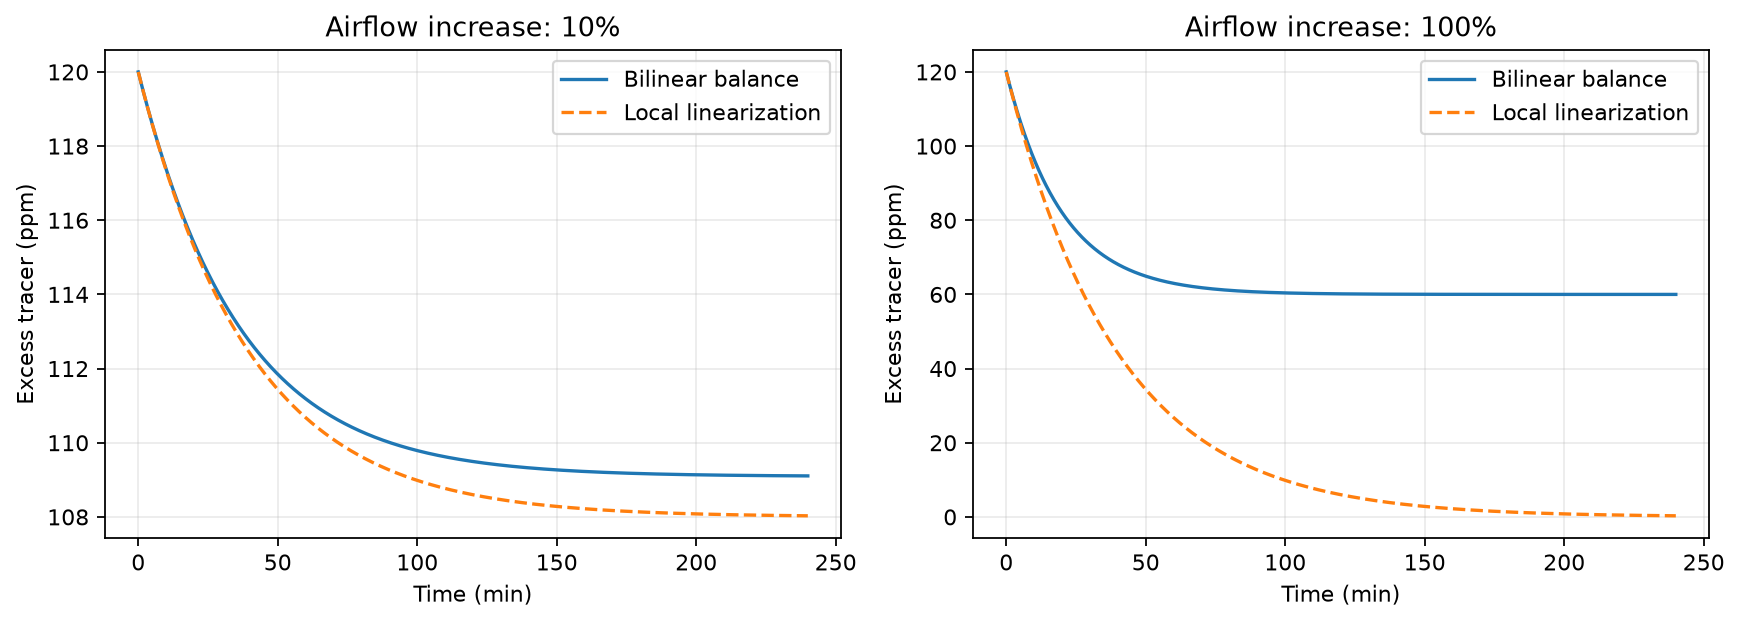
\includegraphics[width=\linewidth,height=.46\textheight,keepaspectratio]{response.png}\end{center}
\section{Method references}
The equations use standard balance laws and feedback-control methods. Further explanation: \url{https://apmonitor.com/pdc/} and \url{https://fbsbook.org/}. Implementation documentation: \url{https://python-control.readthedocs.io/en/0.10.2/}. See the repository reference catalog for individual topics and videos.
\end{document}
